\documentclass[11pt,english,a4paper]{article}

\usepackage[utf8]{inputenc}          % Allows UTF-8 encoded characters in the .tex-file.
\usepackage{babel,csquotes,textcomp} % Set LaTeX to structure the content following international academic standards.
\usepackage[titletoc,toc]{appendix}
\usepackage{subfig}

\usepackage{hyperref}
\usepackage{graphicx}
\usepackage{pdfpages}
\usepackage{listings}
\usepackage{wrapfig}
\usepackage{color,colortbl}
\usepackage{lettrine}
\usepackage[font={small,it}]{caption}
\usepackage{multirow}
\usepackage{tabularx}
\usepackage{footnote}
\usepackage{enumitem}
\usepackage{amsmath}

\usepackage{setspace}
\onehalfspacing

\usepackage[
    backend=biber,
    style=numeric
]{biblatex}
\addbibresource{refs.bib}

\lstset{ %
  basicstyle=\ttfamily\small,     
  backgroundcolor=\color{white},   % choose the background color
  breaklines=true,                 % automatic line breaking only at whitespace
  captionpos=b,                    % sets the caption-position to bottom
  commentstyle=\color{mygreen},    % comment style
  escapeinside={\%*}{*)},          % if you want to add LaTeX within your code
  keywordstyle=\color{blue},       % keyword style
  stringstyle=\color{mymauve},     % string literal style
}

\title{Lab report \\ Frequency Counters}
\author{Aril Schultzen}

\begin{document}
\maketitle
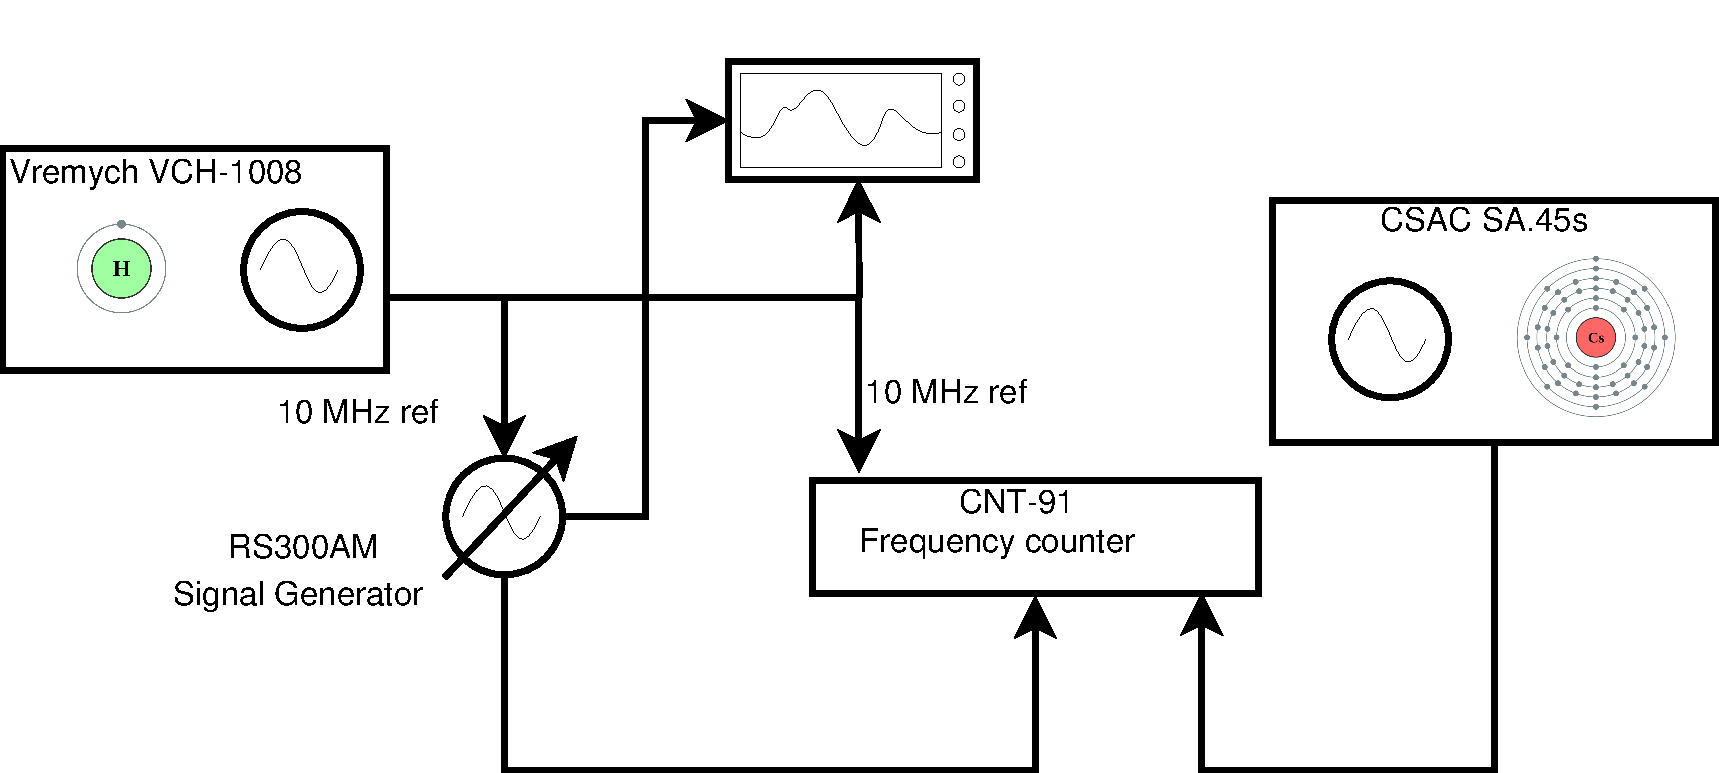
\includegraphics[width=1 \textwidth]{lab_report_diagram.pdf}

\section{Equipment}
\begin{itemize}
  \item Pendulum CNT-91, Frequency counter
  \item Rohde \& Scwarz 300AM, signal generator
  \item Tektronix MD0-4000-6 Oscilloscope
  \item Stopwatch, generic
  \item CSAC, oscillator to measure
  \item Passive Hydrogen maser, frequency reference
  \item RG-58 or RG223 cables
\end{itemize}

\section{Part A, frequency characterization}
\begin{figure}[!htb]
  \centering
  \subfloat[Oscilloscope capture 14:10:41]{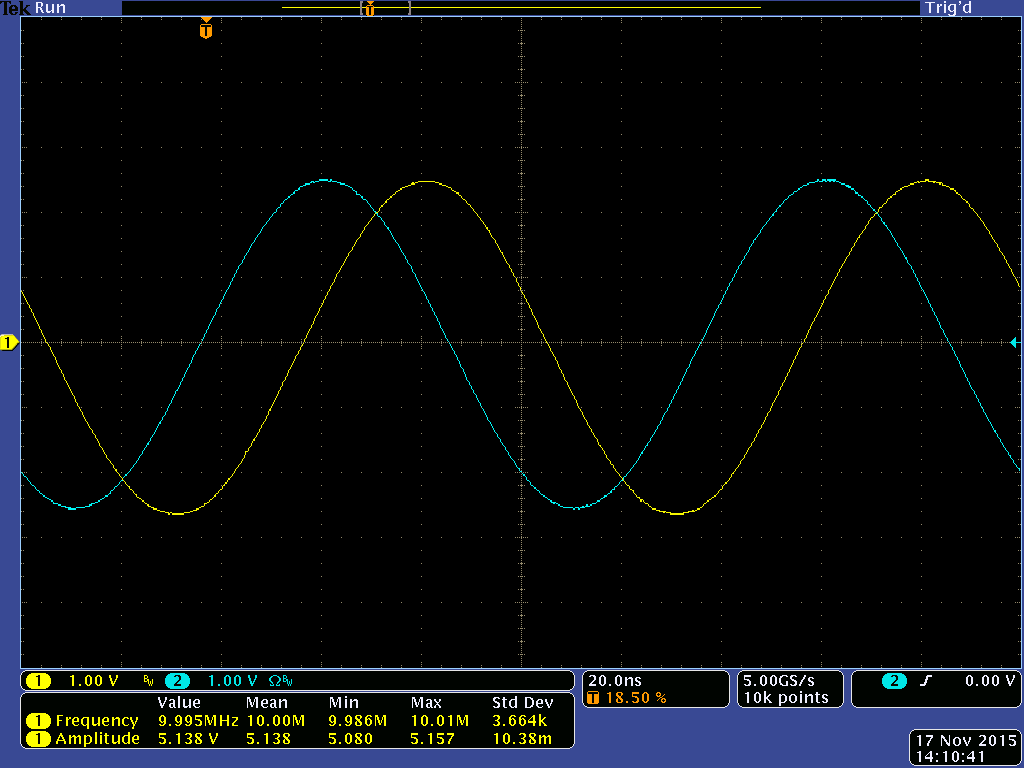
\includegraphics[width=0.5\textwidth]{del_A_kjapp_CSAC.png}\label{fig:f1}}
  \hfill
  \subfloat[Oscilloscope capture 14:10:48]{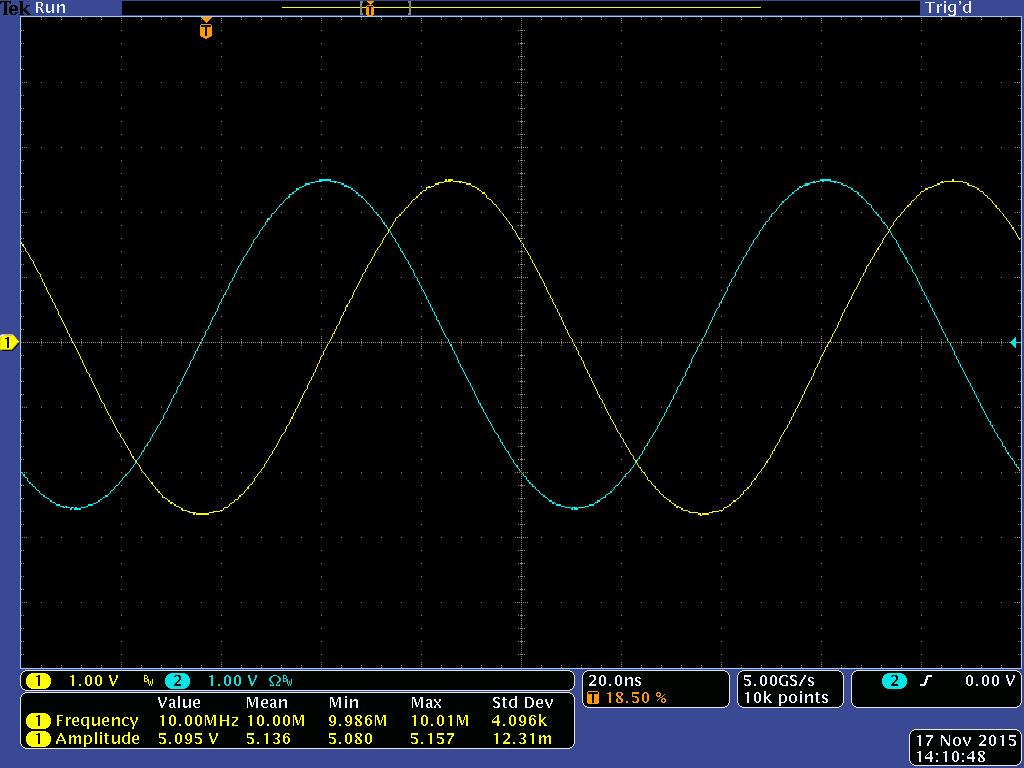
\includegraphics[width=0.5\textwidth]{del_A_kjapp_CSAC2.png}\label{fig:f2}}
  \caption{Oscilloscope captures}
\end{figure}
Figure \ref{fig:f1} and \ref{fig:f2} is two screen shots taken from the oscilloscope. The yellow line is the Passive hydrogen maser, the blue is the CSAC. The oscilloscope is triggering on the input from the CSAC. 

\subsection{Observations}
The two images shows the yellow line moving towards the right, indicating that the CSAC is a bit fast. When set to trigger on the maser instead, the effect is reversed, the blue line moves towards the left. 

\subsection{Measuring relative frequency error}
The period for each of the signals are 100 ns. By measuring the time it took for the two signals to go from being in phase once to twice (in phase, out of phase, in phase again), a relative frequency error can be calculated:

\begin{displaymath}
\frac{period}{phase-in-out-in} = \frac{100 ns}{160 s} = 0,625 ns/s
\end{displaymath}
\newline
It's worth noting that the phase-in-out-in time was measured using my wristwatch and that the accuracy of the measurement was anything but accurate. This is not a problem since the oscillators where measured with extremely high resolution.
The same principle applies to the oscilloscope concerning its lack of external frequency reference.   
\newpage

\section{Part 2: Frequency counting: Resolution and trigger noise: BTB}
The setup was reconfigured:
\begin{center}
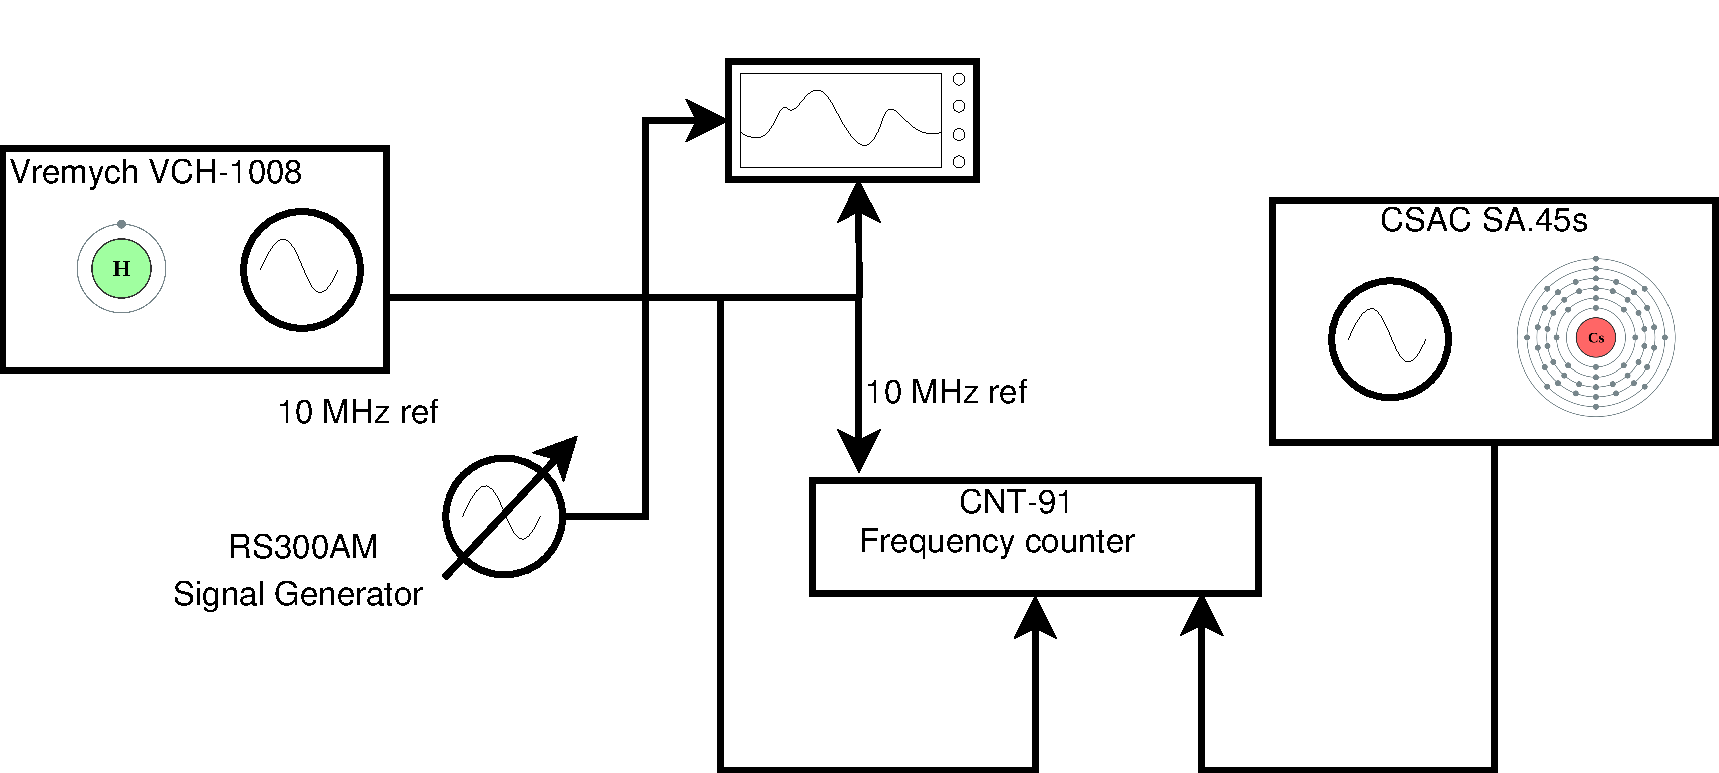
\includegraphics[width=1 \textwidth]{lab_report_diagram_del2.pdf}
\end{center}
The frequency counter now measures the maser (on input A) and uses it as reference. TimeView was then used to measure the frequency on input A, doing 200 samples with 1 s interval.

\subsection{Observations}
\subsubsection{Trigger resolution}
According to the User Manual for the CNT 9x Series, the resolution for Period A,B Back-to-Back is 50 ps rms. By observing the Allan deviation for the measurement (\ref{fig:allan_dev1}) the same can be observed: At the 1 second mark, the Allan Deviation is 8.23E-11 (around 82,3 ps) which seems about right considering start and stop at 50 ps (each) rms. Considering the slope, we are dealing with white phase and flicker noise (-1 slope). When studying the Modified Allan deviation for the same data (\ref{fig:mod_allan_dev1}), it becomes clear that the dominant type of noise is white noise (-3/2 slope).

\begin{figure}[]
  \caption{Allan deviation for 200 samples at 1 s sample rate of 10MHz from the Passive Hydrogen maser.}
  \centering
    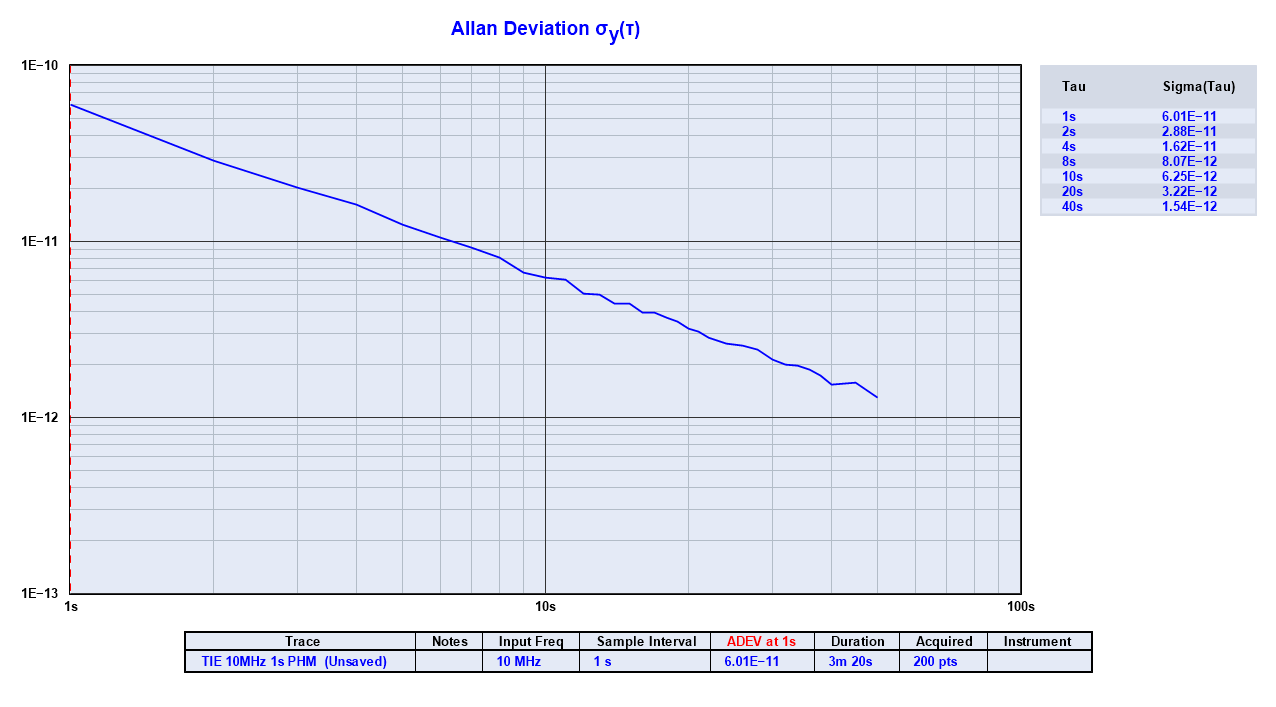
\includegraphics[width=1\textwidth]{phm10mhz1s_allan.png}
    \label{fig:allan_dev1}
\end{figure}

\begin{figure}[]
  \caption{Modified Allan deviation for 200 samples at 1 s sample rate of 10MHz from the Passive Hydrogen maser.}
  \centering
    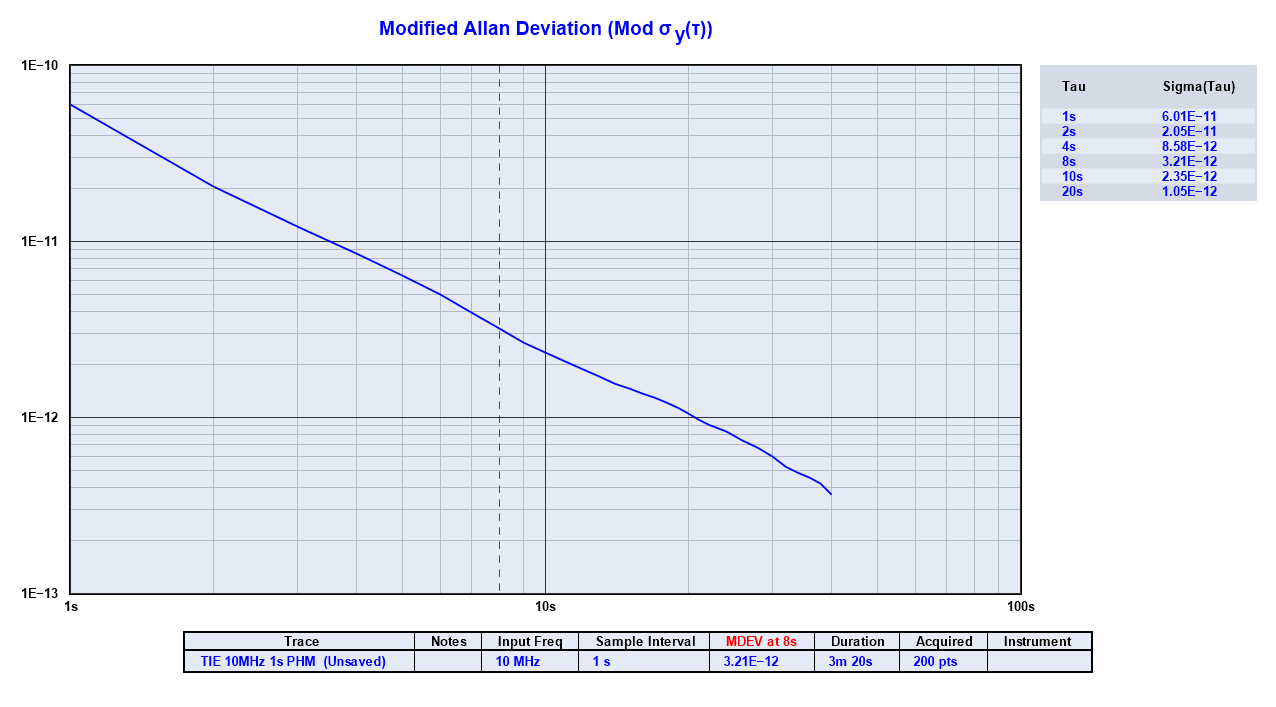
\includegraphics[width=1\textwidth]{phm10mhz1s_modified_allan.png}
    \label{fig:mod_allan_dev1}
\end{figure}

\newpage
\subsubsection{Trigger level}
\begin{wrapfigure}{c}{0.45\textwidth}
  \centering
  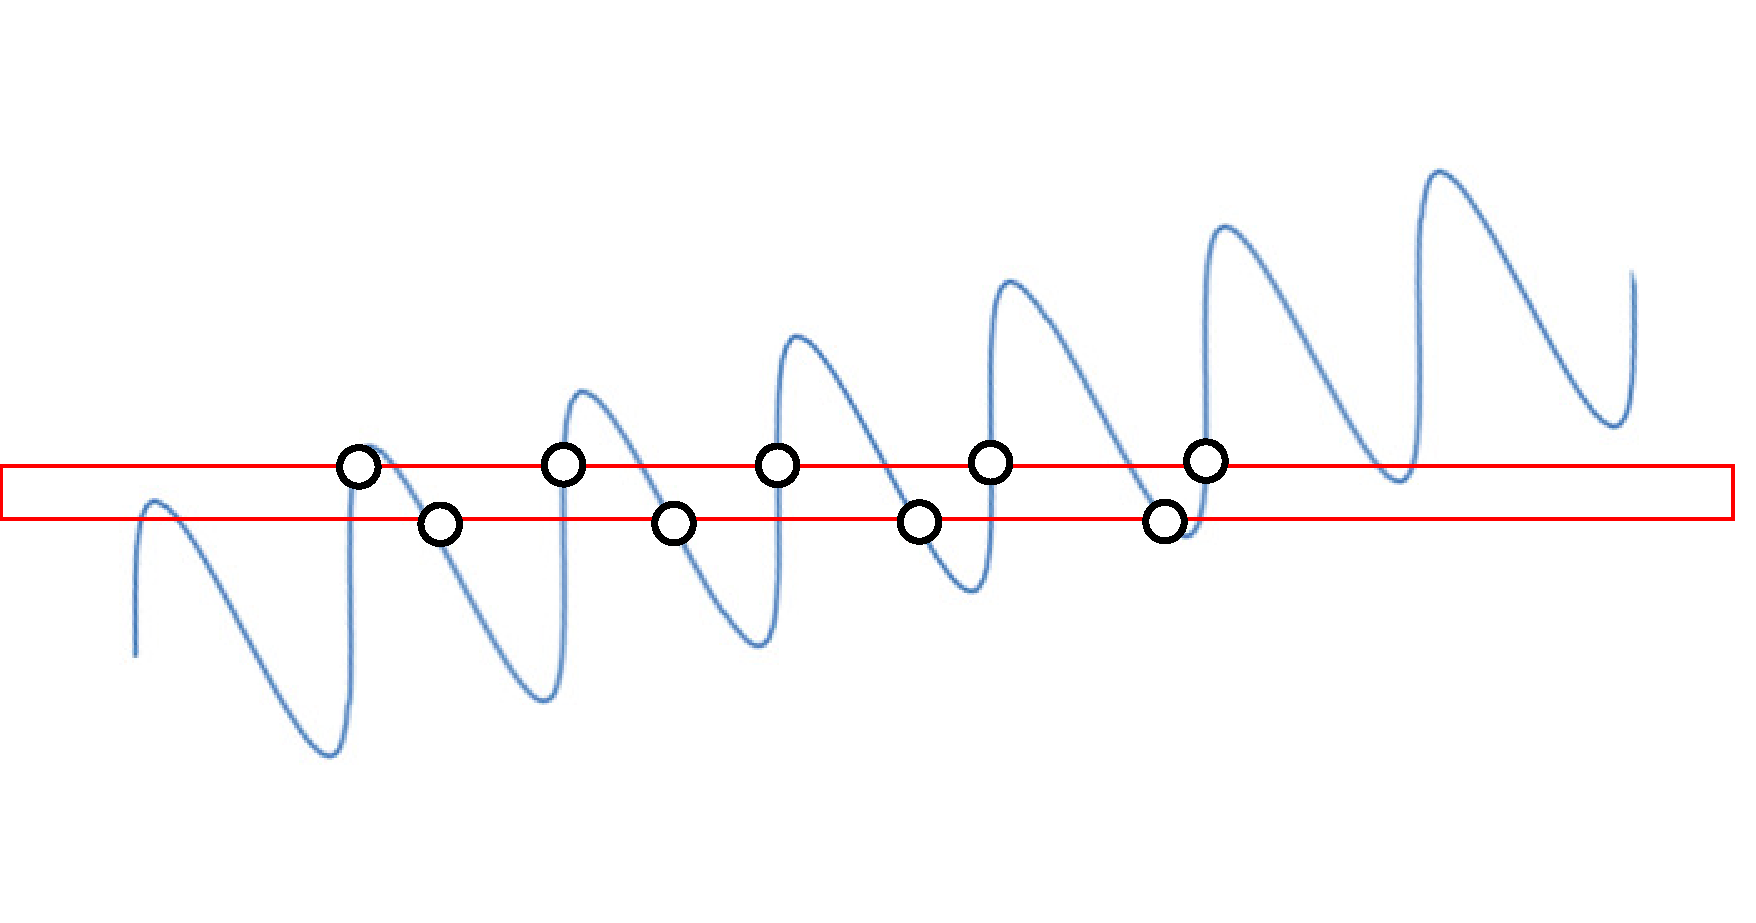
\includegraphics[width=0.40\textwidth]{hysteresis.pdf}
  \caption{Trigger counting multiple times as noise passes the hysteresis window}
    \label{fig:hysteresis}
\end{wrapfigure}
When raising the trigger level from 0 V to 1.2 V, more noise is introduced. This is because the slope of the signal is steeper at 0 V than at 1.2 V (closer to the middle of the sine wave) This means the signal is passing the hysteresis window at lower speed. The lower slope results in a less accurate trigging. In a really noisy signal, the signal can pass the hysteresis window more than once, thus generating erroneous counts (see figure \ref{fig:hysteresis}). 

\section{Part 2: Frequency counting: Resolution and trigger noise: TIE}
One of the advantages of the Modified Allan Deviation relative to regular Allan variance, is the ability to separate white phase noise from flicker noise. As we saw earlier, the dominating noise introduced by our frequency counter, was white noise. This noise is possible to reduce by calculating a running average as shown by the blue line in figure \ref{fig:PHM_10MHz_allan_dev}. The pink line is drawn from the same data but without the averaging technique. When observing the Modified Allan Deviance (as shown in figure \ref{fig:PHM_10MHz_mod_allan_dev}), it becomes apparent that the averaging has removed some of the white noise that earlier dominated. The flicker noise however, is still there as clearly shown at the 1 second mark. 

\begin{figure}[!htb]
  \centering
  \subfloat[Cut out of screen shot showing the frequency difference for the measurement.]{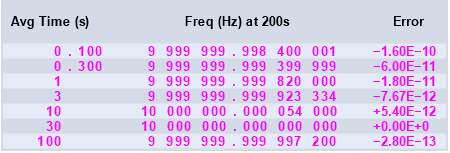
\includegraphics[width=0.5\textwidth]{tie_10mhz_phm_1ms_freq_diff_utklipp.png}\label{fig:freq_diff1}}
  \hfill
  \subfloat[Same cut out, but for the smoothed measurements. This measurement is clearly better.]{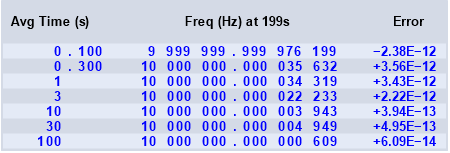
\includegraphics[width=0.5\textwidth]{tie_10mhz_phm_1ms_smooth_freq_diff_utklipp.png}\label{fig:freq_diff2}}
\end{figure}
As figure \ref{fig:freq_diff1} and \ref{fig:freq_diff2} shows, using an averaging technique when conducting measurements is obviously effective against white phase noise.

\begin{figure}[!htb]
  \caption{TIE 10MHz PHM 1 ms sample rate Allan Deviation.}
  \centering
    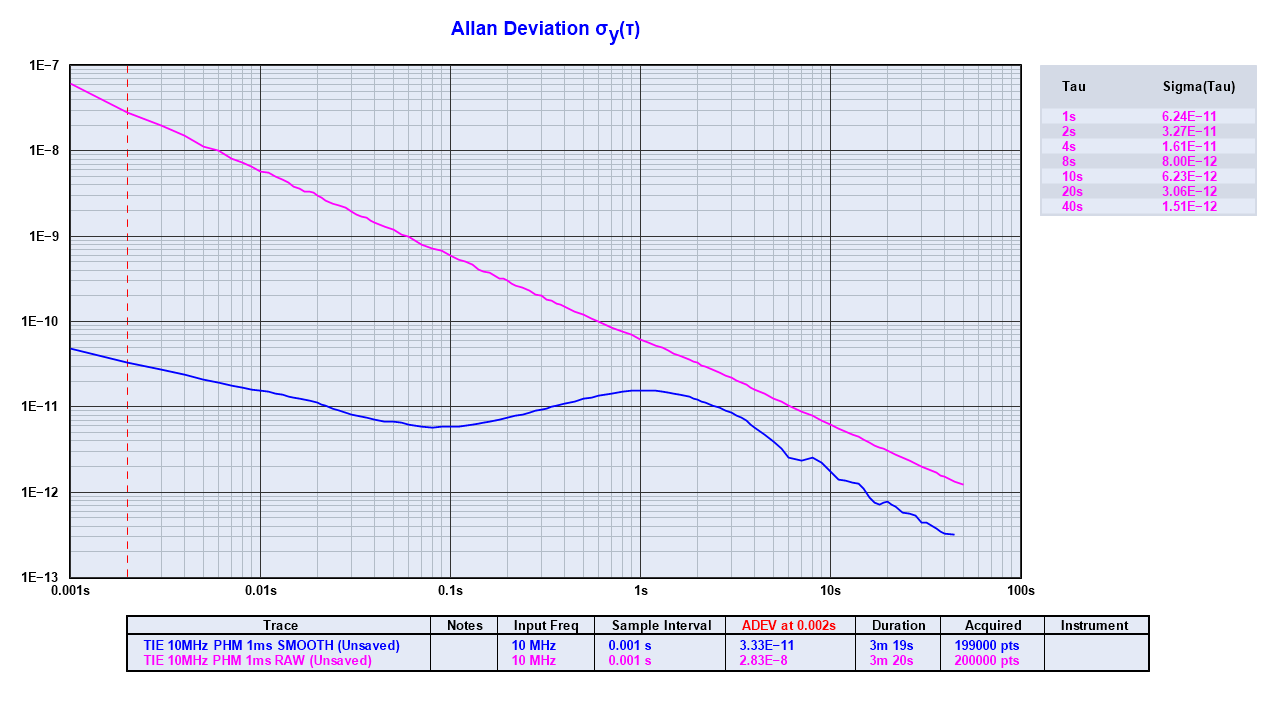
\includegraphics[width=1\textwidth]{tie_10mhz_phm_1ms_allan.png}
    \label{fig:PHM_10MHz_allan_dev}
\end{figure}

\begin{figure}[!htb]
  \caption{TIE 10MHz PHM 1 ms sample rate Modified Allan Deviation.}
  \centering
    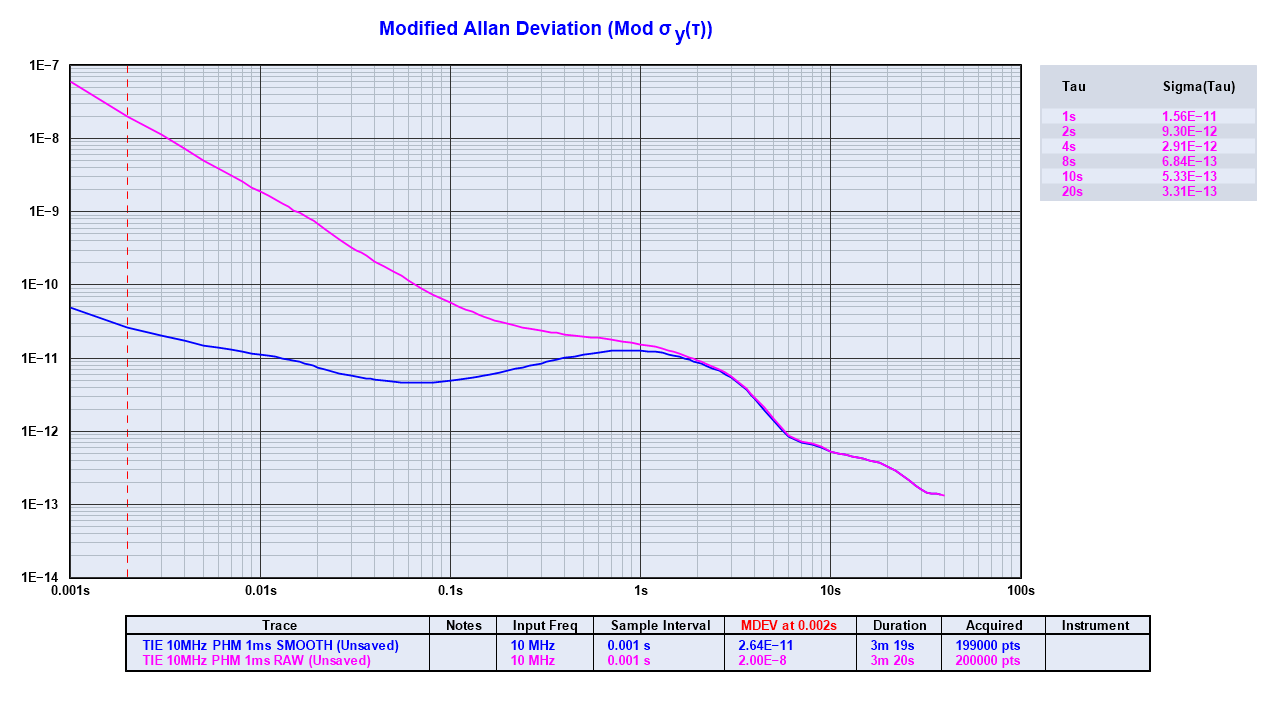
\includegraphics[width=1\textwidth]{tie_10mhz_phm_1ms_modified_allan.png}
    \label{fig:PHM_10MHz_mod_allan_dev}
\end{figure}

\newpage
\section{Part 3: Frequency counting: Resolution and trigger noise: KHz and MHz}
The setup was reset to it's initial configuration. 
\begin{figure}[!htb]
  \caption{Screen shot showing the frequency difference of fbtb 10MHz and 10Khz from the signal generator}
  \centering
    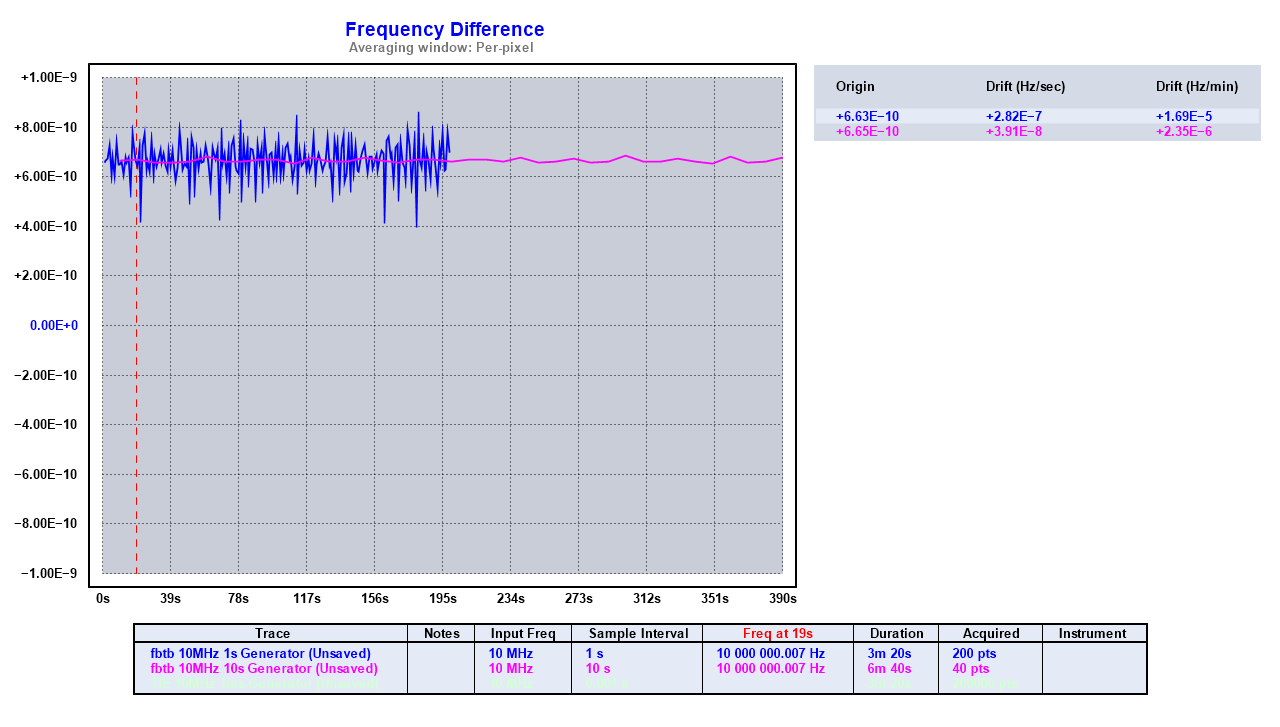
\includegraphics[width=1\textwidth]{freq_diff_del3.png}
    \label{fig:freq_diff_3}
\end{figure}
As figure \ref{fig:freq_diff_3} suggests, our earlier measurements using a wristwatch to determine the relative frequency error seems to be correct. These measurements though naive, is pretty accurate relative to the offset that the signal generator was configured to apply (+6.66E-10). By studying the Allan Deviation and the Modified Allan Deviation for the measurement, it becomes clear that using a sample rate of 10 seconds as opposed to 1 s, results in a more accurate measurement. The reason for this is that the trigger error divided by time is reduced when doing fewer measurements. Once again, the "Achilles Heel" of the setup seems to be the frequency counter. 

\begin{figure}[!htb]
  \caption{FBTB 10MHz/10KHz signal generator at 1/10 s sample rate Allan Deviation.}
  \centering
    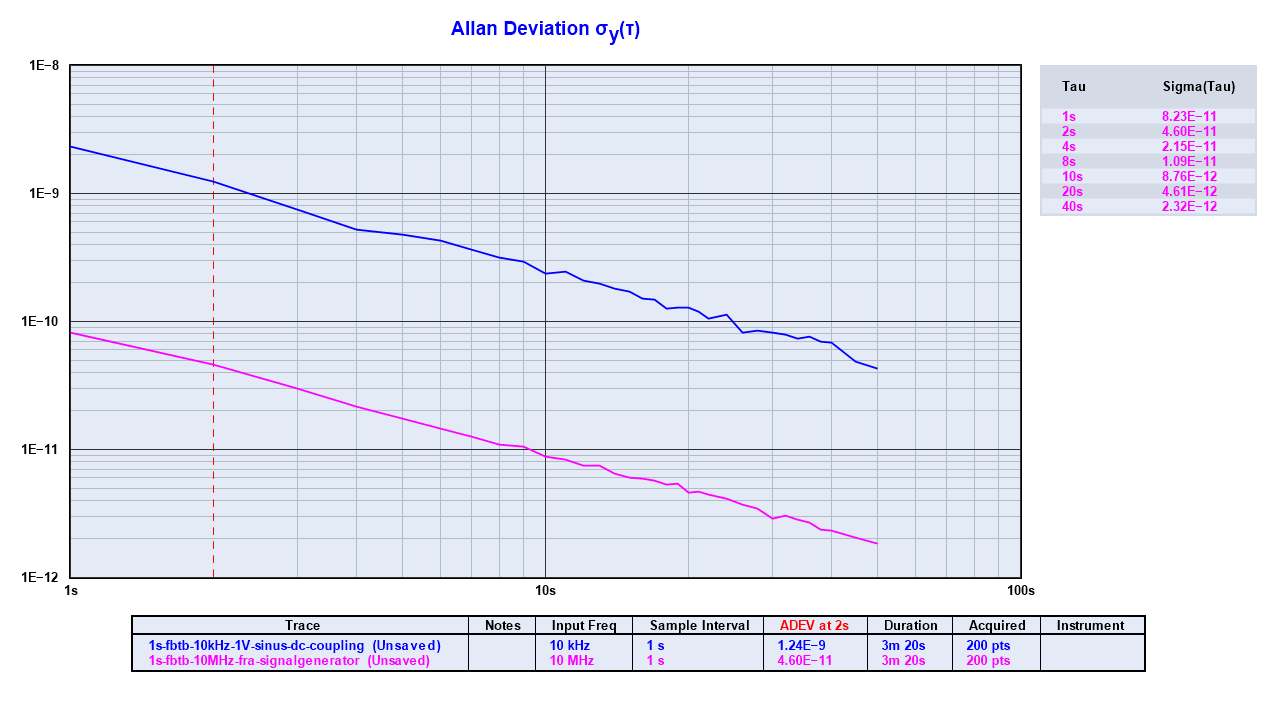
\includegraphics[width=1\textwidth]{fbtb_10mhzkhz_generator_allan.png}
    \label{fig:sg_10x_allan_dev}
\end{figure}

\begin{figure}[!htb]
  \caption{FBTB 10MHz/10Khz signal generator at 1/10 s sample rate Modified Allan Deviation.}
  \centering
    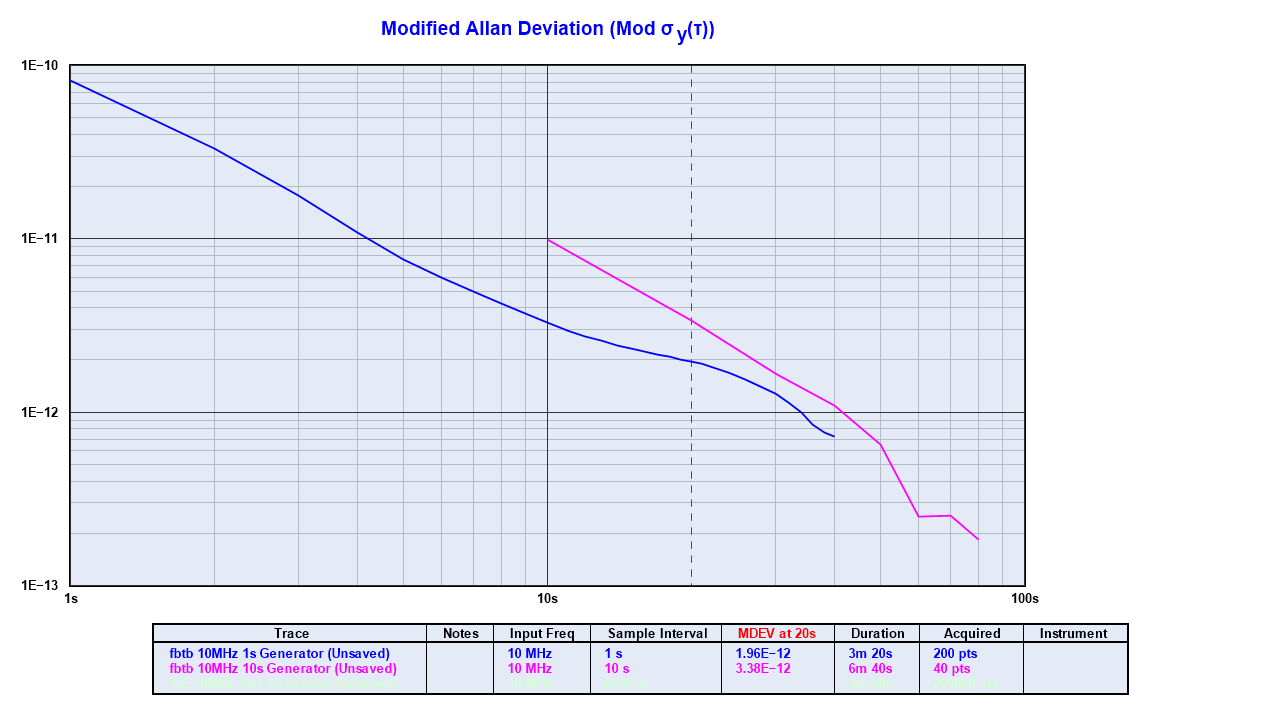
\includegraphics[width=1\textwidth]{fbtb_10mhzkhz_generator_mod_allan.png}
    \label{fig:sg_10x_mod_allan_dev}
\end{figure}

Figure \ref{fig:sg_10x_mod_allan_dev} is a screen shot of the Modified Allan Deviation for the following measurements:
\begin{itemize}
  \item TIE 10 KHz 1 ms sample rate 1V (blue)
  \item TIE 10 MHz 1 ms sample rate 5V (pink)
  \item TIE 10 KHz 1 ms sample rate 1V Smoothed (for good measure) (green)
\end{itemize}
The figure seems to suggest that having an higher amplitude thus passing the hysteresis window faster, results in less flicker noise because the triggers job becomes easier. This is however just my theory as the lab experiment at this point was side tracked by a weird "bar-code" phenomena.

\begin{figure}[!htb]
  \caption{TIE measurements for 10 MHz/KHz 1 ms sample rate 1/5V Modified Allan Deviation}
  \centering
    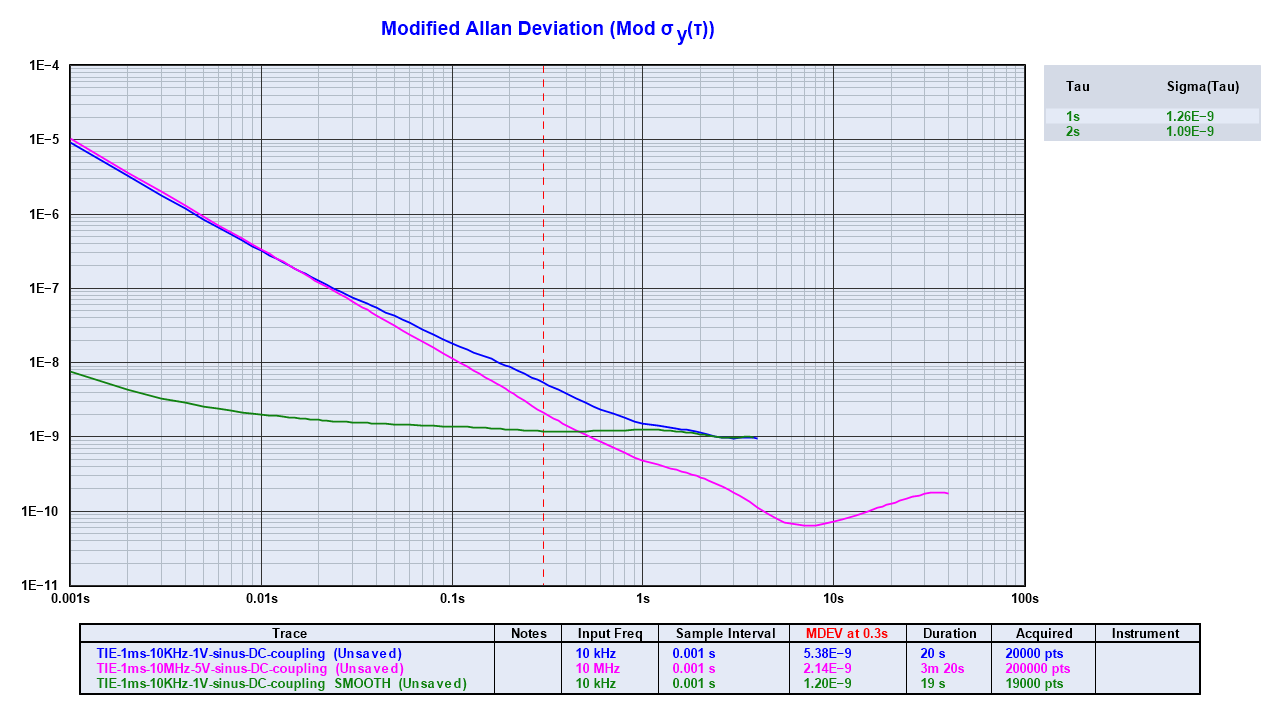
\includegraphics[width=1\textwidth]{mod_allan_last_part3.png}
    \label{fig:sg_10x_mod_allan_dev}
\end{figure}


\end{document}                     